\documentclass[12pt,notitlepage,letterpaper]{article}
\usepackage[margin=0.5in]{geometry}
\usepackage[utf8]{inputenc}
\usepackage{amsmath,amsfonts,amssymb,graphicx}
\usepackage{tikz}

\begin{document}
\title{Inter-Device Sharing}
\date{}
\maketitle

\section{Overview}

\section{Sharing flow between UI and backend}
To initiate a share operation, the UI implementation will call into the backend
code, which will prepare the data for transmission, launch a background thread
to handle incoming clients, and generate a QR code, which will be passed back to
the UI thread as a \texttt{Drawable}.

Once the background process has launched, notifications of errors or successful
transmission will be sent to the UI thread via a passed handler object, if one
was given.

\begin{figure}[h]\centering
    \caption{UI/Backend Sharing Process}
    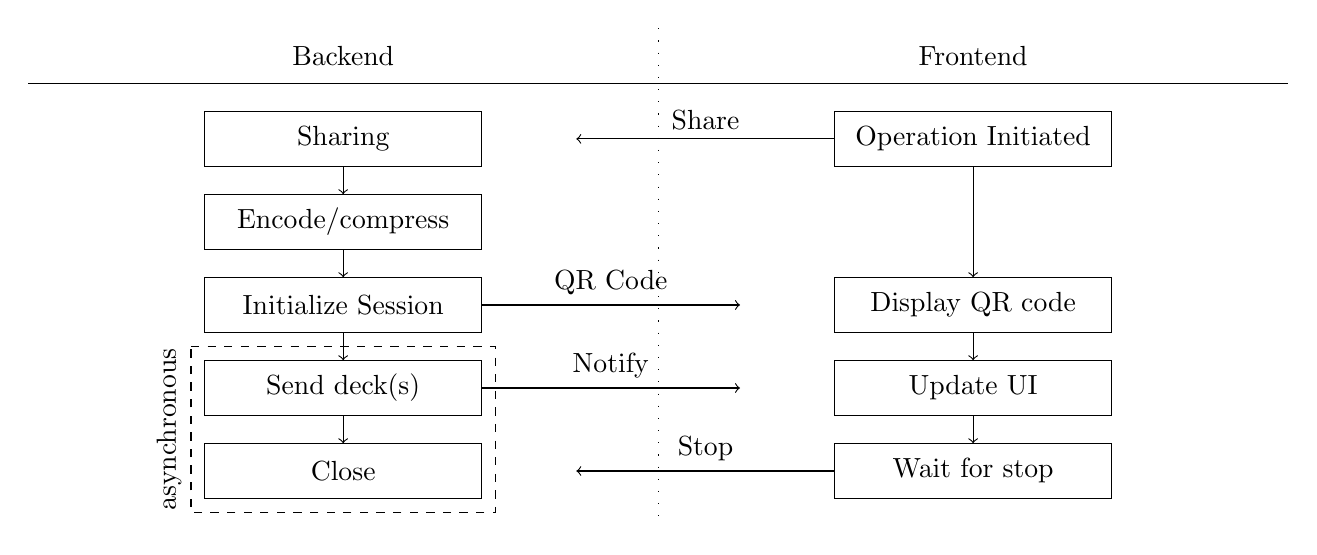
\begin{tikzpicture}
        \draw (0,0) -- (16,0);
        \draw[loosely dotted] (8,2em) -- (8,-16em);
        \draw (4,1em) node {Backend}
              (12,1em) node {Frontend};
        \node (Bsharing)    at (4,-2em)  [draw,minimum height=2em,minimum width=10em] {Sharing};
        \node (Bencode)     at (4,-5em)  [draw,minimum height=2em,minimum width=10em] {Encode/compress};
        \node (Bsessinit)   at (4,-8em)  [draw,minimum height=2em,minimum width=10em] {Initialize Session};
        \node (Bsenddeck)   at (4,-11em) [draw,minimum height=2em,minimum width=10em] {Send deck(s)};
        \node (Bclose)      at (4,-14em) [draw,minimum height=2em,minimum width=10em] {Close};
        \node (Finit)       at (12,-2em)  [draw,minimum height=2em,minimum width=10em] {Operation Initiated};
        \node (Fqrui)       at (12,-8em)  [draw,minimum height=2em,minimum width=10em] {Display QR code};
        \node (Fnotified)   at (12,-11em)  [draw,minimum height=2em,minimum width=10em] {Update UI};
        \node (Fstopped)    at (12,-14em) [draw,minimum height=2em,minimum width=10em] {Wait for stop};

        \draw[->] (Finit) ++(0,-1em) -- ++(0,-4em);
        \draw[->] (Fqrui) ++(0,-1em) -- ++(0,-1em);
        \draw[->] (Fnotified) ++(0,-1em) -- ++(0,-1em);

        \draw[->] (Bsharing) ++(0,-1em) -- ++(0,-1em);
        \draw[->] (Bencode) ++(0,-1em) -- ++(0,-1em);
        \draw[->] (Bsessinit) ++(0,-1em) -- ++(0,-1em);
        \draw[->] (Bsenddeck) ++(0,-1em) -- ++(0,-1em);

        \draw[->] (Finit) ++(-5em,0) -- ++(-9.34em,0) node[pos=0.5,above]{Share};
        \draw[->] (Bsessinit) ++(5em,0) -- ++(9.34em,0) node[pos=0.5,above]{QR Code};
        \draw[->] (Bsenddeck) ++(5em,0) -- ++(9.34em,0) node[pos=0.5,above]{Notify};
        \draw[->] (Fstopped) ++(-5em,0) -- ++(-9.34em,0) node[pos=0.5,above]{Stop};

        \draw[dashed] (Bsenddeck) ++(-5.5em,1.5em) -- ++(11em,0)
                                                   -- ++(0, -6em)
                                                   -- ++(-11em,0)
                                                   -- cycle
                                                   node[pos=0.5,above,rotate=90]{asynchronous};
    \end{tikzpicture}
\end{figure}

\pagebreak\section{Sharing flow between server and client devices}
\begin{figure}[h]\centering
    \caption{Inter-Device Sharing Process}
    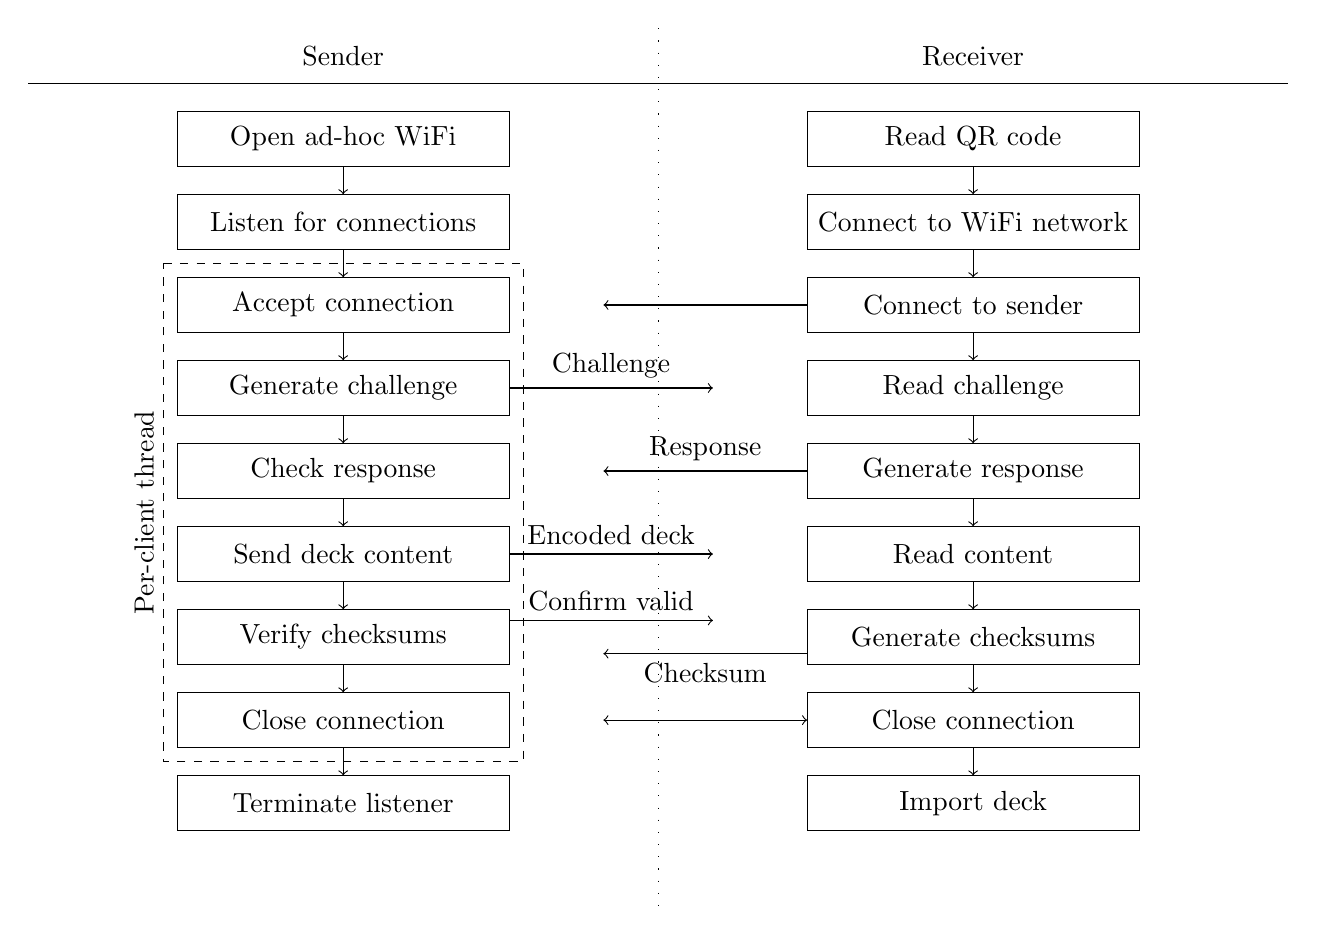
\begin{tikzpicture}
        \draw (0,0) -- (16,0);
        \draw[loosely dotted] (8,2em) -- (8,-30em);
        \draw (4,1em) node {Sender} (12,1em) node {Receiver};

        \node (Sopenwifi)   at (4,-2em)  [draw,minimum height=2em,minimum width=12em] {Open ad-hoc WiFi};
        \node (Slisten)     at (4,-5em)  [draw,minimum height=2em,minimum width=12em] {Listen for connections};
        \node (Saccept)     at (4,-8em)  [draw,minimum height=2em,minimum width=12em] {Accept connection};
        \node (Schallenge)  at (4,-11em) [draw,minimum height=2em,minimum width=12em] {Generate challenge};
        \node (Scheck)      at (4,-14em) [draw,minimum height=2em,minimum width=12em] {Check response};
        \node (Ssend)       at (4,-17em) [draw,minimum height=2em,minimum width=12em] {Send deck content};
        \node (Sverify)     at (4,-20em) [draw,minimum height=2em,minimum width=12em] {Verify checksums};
        \node (Sclose)      at (4,-23em) [draw,minimum height=2em,minimum width=12em] {Close connection};
        \node (Sterm)       at (4,-26em) [draw,minimum height=2em,minimum width=12em] {Terminate listener};

        \node (Rreadqr)     at (12,-2em)  [draw,minimum height=2em,minimum width=12em] {Read QR code};
        \node (Rwifi)       at (12,-5em)  [draw,minimum height=2em,minimum width=12em] {Connect to WiFi network};
        \node (Rconnect)    at (12,-8em)  [draw,minimum height=2em,minimum width=12em] {Connect to sender};
        \node (Rreadchal)   at (12,-11em) [draw,minimum height=2em,minimum width=12em] {Read challenge};
        \node (Rrespond)    at (12,-14em) [draw,minimum height=2em,minimum width=12em] {Generate response};
        \node (Rread)       at (12,-17em) [draw,minimum height=2em,minimum width=12em] {Read content};
        \node (Rgenhash)    at (12,-20em) [draw,minimum height=2em,minimum width=12em] {Generate checksums};
        \node (Rclose)      at (12,-23em) [draw,minimum height=2em,minimum width=12em] {Close connection};
        \node (Rimport)     at (12,-26em) [draw,minimum height=2em,minimum width=12em] {Import deck};

        % Vertical sequence arrows
        \foreach \x in {Rreadqr,Rwifi,Rconnect,Rreadchal,Rrespond,Rread,Rgenhash,Rclose}
            \draw[->] (\x) ++(0,-1em) -- ++(0,-1em);
        \foreach \x in {Sopenwifi,Slisten,Saccept,Schallenge,Scheck,Ssend,Sverify,Sclose}
            \draw[->] (\x) ++(0,-1em) -- ++(0,-1em);

        % Cross-process arrows
        \draw[->] (Rconnect) ++ (-6em,0) -- ++(-7.36em,0) node[pos=0.5,above]{};
        \draw[->] (Schallenge) ++ (6em,0) -- ++(7.36em,0) node[pos=0.5,above]{Challenge};
        \draw[->] (Rrespond) ++ (-6em,0) -- ++(-7.36em,0) node[pos=0.5,above]{Response};
        \draw[->] (Ssend) ++ (6em,0) -- ++(7.36em,0) node[pos=0.5,above]{Encoded deck};
        \draw[->] (Rgenhash) ++ (-6em,-0.6em) -- ++(-7.36em,0) node[pos=0.5,below]{Checksum};
        \draw[->] (Sverify) ++ (6em,0.6em) -- ++(7.36em,0) node[pos=0.5,above]{Confirm valid};
        \draw[<->] (Rclose) ++ (-6em,0) -- ++(-7.36em,0);

        % Draw dotted box around per-client server thread
        \draw[dashed] (Saccept)++(-6.5em,1.5em) -- ++(13em,0)
                                                -- ++(0,-18em)
                                                -- ++(-13em,0)
                                                -- cycle
                                                node[pos=0.5,above,rotate=90]
                                                {Per-client thread};
    \end{tikzpicture}
\end{figure}

\section{QR Code format}
The QR Code used for encryption key and wireless credential transmission is a
Version 6 at ECC level Q. This code can store 74 bytes of binary data, of which
the first 16 are the host's randomly-generated SSID, the next 32 are a 256-bit
AES key used to secure data during transmission, and the remainder is a
variable-length field (padded with null bytes after the data ends) containing the
random network password.

Rather than include an internal checksum, the format relies on the checksum and
error correction of the containing QR code to ensure that data is transmitted
correctly.

\section{Network protocol}

\section{Security and Authentication}

\end{document}
